\documentclass[11pt]{article}
\usepackage[margin=1in]{geometry}
\usepackage{amsmath,amssymb}
\usepackage{graphicx}
\usepackage{booktabs}
\usepackage{enumitem}
\usepackage{xcolor}
\usepackage{listings}
\usepackage{float}
\usepackage{tikz}
\usepackage{hyperref}

\lstset{basicstyle=\ttfamily\scriptsize, keywordstyle=\color{blue!70!black},
        stringstyle=\color{red!60!black}, language=Python, frame=single, breaklines=true, numbers=left,
        numberstyle=\tiny\color{gray}, columns=fullflexible, showstringspaces=false}

\title{EECE 5639: Computer Vision\\Fall 2026, Homework 3}
\author{Jingqi Mei}
\date{October 23, 2026}

\setlength{\emergencystretch}{3em}
\setlength{\parindent}{0pt}
\setlength{\parskip}{4pt}
\begin{document}
\maketitle

Normal form of a line: $x\cos\theta + y\sin\theta = \rho$, where $\rho$ is the signed distance and $0^\circ\le\theta<180^\circ$.

%=====================================================================
\section*{Question 1}
%=====================================================================
\subsection*{(a)}
\begin{itemize}[leftmargin=*]
\item $AB$: $A=(2,0)$, $B=(2,2)$, so the line is $x=2$. \quad $\Rightarrow (\rho_1,\theta_1) = (2,\;0^\circ)$
\item $BC$: $B=(2,2)$, $C=(0,2)$, so the line is $y=2$. \quad $\Rightarrow (\rho_2,\theta_2) = (2,\;90^\circ)$
\item $CA$: $C=(0,2)$, $A=(2,0)$, so the line is $x+y=2$. Dividing by $\sqrt2$ gives $x\cos45^\circ+y\sin45^\circ=\sqrt2$. \quad $\Rightarrow (\rho_3,\theta_3) = (\sqrt2,\;45^\circ)$
\end{itemize}

\subsection*{(b)}
\begin{center}
\begin{tabular}{lcccc}\toprule
Line & $(\rho_i,\theta_i)$ & $(\rho_i^2,\;\theta_i+90^\circ)$ & $(\rho_i',\theta_i')$ in range & Equation\\\midrule
1 & $(2,0^\circ)$ & $(4,90^\circ)$ & $(4,90^\circ)$ & $y=4$\\
2 & $(2,90^\circ)$ & $(4,180^\circ)$ & $(-4,0^\circ)$ & $x=-4$\\
3 & $(\sqrt2,45^\circ)$ & $(2,135^\circ)$ & $(2,135^\circ)$ & $-x+y=2\sqrt2$\\\bottomrule
\end{tabular}
\end{center}
Line 2 has $\theta=180^\circ$, which is outside the range. Since $(\rho,\theta)$ and $(-\rho,\theta-180^\circ)$ describe the same line, it becomes $(-4,0^\circ)$.

Intersecting the three lines gives the vertices:
\begin{align*}
A'&=L_1\cap L_2=(-4,\,4),\\
B'&=L_1\cap L_3=(4-2\sqrt2,\;4)\approx(1.17,\,4),\\
C'&=L_2\cap L_3=(-4,\;2\sqrt2-4)\approx(-4,\,-1.17).
\end{align*}

\begin{figure}[H]\centering
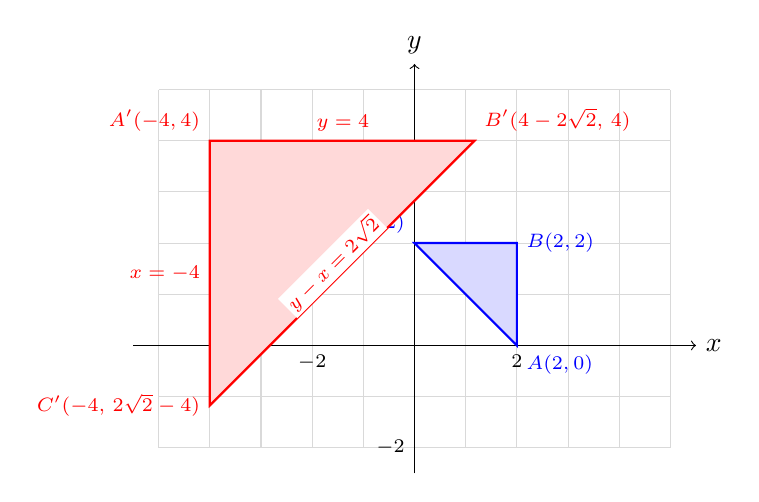
\begin{tikzpicture}[scale=0.65]
  \draw[gray!30] (-5,-2) grid (5,5);
  \draw[->] (-5.5,0) -- (5.5,0) node[right] {$x$};
  \draw[->] (0,-2.5) -- (0,5.5) node[above] {$y$};
  \foreach \t in {-2,2} \node[below,font=\scriptsize] at (\t,0) {$\t$};
  \foreach \t in {-2} \node[left,font=\scriptsize] at (0,\t) {$\t$};
  \fill[blue!15] (2,0) -- (2,2) -- (0,2) -- cycle;
  \draw[blue,thick] (2,0) -- (2,2) -- (0,2) -- cycle;
  \node[blue,below right,font=\scriptsize] at (2,0) {$A(2,0)$};
  \node[blue,right,font=\scriptsize] at (2,2) {$B(2,2)$};
  \node[blue,above left,font=\scriptsize] at (0,2) {$C(0,2)$};
  \fill[red!15] (-4,4) -- (1.1716,4) -- (-4,-1.1716) -- cycle;
  \draw[red,thick] (-4,4) -- (1.1716,4) -- (-4,-1.1716) -- cycle;
  \node[red,above left,font=\scriptsize] at (-4,4) {$A'(-4,4)$};
  \node[red,above right,font=\scriptsize] at (1.1716,4) {$B'(4-2\sqrt2,\,4)$};
  \node[red,left,font=\scriptsize] at (-4,-1.1716) {$C'(-4,\,2\sqrt2-4)$};
  \node[red,above,font=\scriptsize] at (-1.4,4) {$y=4$};
  \node[red,left,font=\scriptsize] at (-4,1.4) {$x=-4$};
  \node[red,rotate=45,font=\scriptsize,fill=white,inner sep=1pt] at (-1.6,1.6) {$y-x=2\sqrt2$};
\end{tikzpicture}
\caption{Original triangle (blue) and modified triangle (red).}
\end{figure}

\subsection*{(c)}
\begin{itemize}[leftmargin=*]
\item Original: a right triangle at $B$ with legs $|AB|=|BC|=2$, so the area is $\tfrac12\cdot2\cdot2 = \mathbf{2}$.
\item Modified: a right triangle at $A'$ with legs $|A'B'| = |A'C'| = 8-2\sqrt2$, so the area is
\[
\tfrac12\left(8-2\sqrt2\right)^2 = \mathbf{36-16\sqrt2 \approx 13.37}.
\]
\end{itemize}

%=====================================================================
\section*{Question 2}
%=====================================================================
\subsection*{(a)}
The four lines are:
\begin{itemize}[leftmargin=*]
\item $AB$: $y=3$
\item $BC$: $x=3$
\item $CD$: $\tfrac12x+\tfrac{\sqrt3}{2}y=\sqrt3$, i.e.\ $x+\sqrt3\,y=2\sqrt3$
\item $DA$: $-\tfrac{1}{\sqrt2}x+\tfrac{1}{\sqrt2}y=\tfrac1{\sqrt2}$, i.e.\ $y=x+1$
\end{itemize}
The vertices are the intersections of adjacent sides:
\begin{align*}
A &= DA\cap AB = (2,\,3), & B &= AB\cap BC = (3,\,3),\\
C &= BC\cap CD = (3,\;2-\sqrt3)\approx(3,\,0.27), & D &= CD\cap DA = \left(\tfrac{3-\sqrt3}{2},\;\tfrac{5-\sqrt3}{2}\right)\approx(0.63,\,1.63).
\end{align*}

\begin{figure}[H]\centering
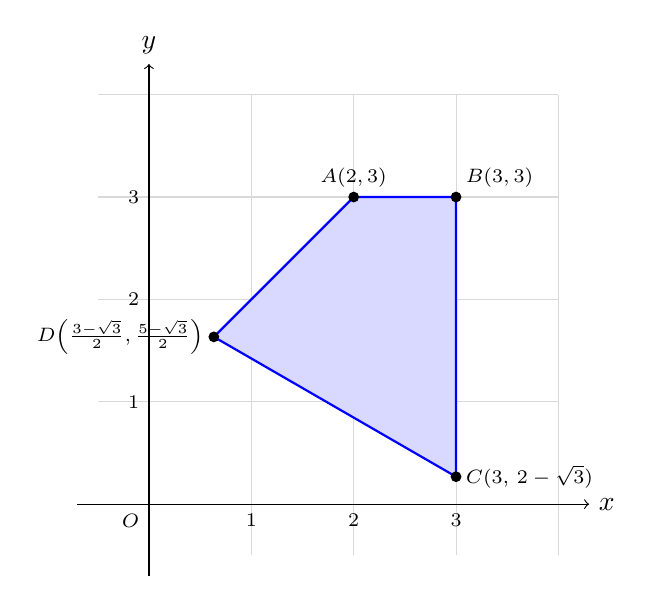
\begin{tikzpicture}[scale=1.3]
  \draw[gray!30] (-0.5,-0.5) grid (4,4);
  \draw[->] (-0.7,0) -- (4.3,0) node[right] {$x$};
  \draw[->] (0,-0.7) -- (0,4.3) node[above] {$y$};
  \foreach \t in {1,2,3} {\node[below,font=\scriptsize] at (\t,0) {$\t$}; \node[left,font=\scriptsize] at (0,\t) {$\t$};}
  \node[below left,font=\scriptsize] at (0,0) {$O$};
  \fill[blue!15] (2,3) -- (3,3) -- (3,0.2679) -- (0.6340,1.6340) -- cycle;
  \draw[blue,thick] (2,3) -- (3,3) -- (3,0.2679) -- (0.6340,1.6340) -- cycle;
  \foreach \p in {(2,3),(3,3),(3,0.2679),(0.6340,1.6340)} \fill \p circle (1.5pt);
  \node[above,font=\scriptsize] at (2,3) {$A(2,3)$};
  \node[above right,font=\scriptsize] at (3,3) {$B(3,3)$};
  \node[right,font=\scriptsize] at (3,0.2679) {$C(3,\,2-\sqrt3)$};
  \node[left,font=\scriptsize] at (0.6340,1.6340) {$D\!\left(\frac{3-\sqrt3}{2},\frac{5-\sqrt3}{2}\right)$};
\end{tikzpicture}
\caption{The convex polygon $ABCD$.}
\end{figure}

\subsection*{(b)}
Let $\mathbf n_\theta=(\cos\theta,\sin\theta)$. A point $\mathbf p$ is on the line when $\mathbf n_\theta\cdot\mathbf p=\rho$. Rotating by $90^\circ$ gives $R\mathbf p$, and $\mathbf n_{\theta+90^\circ}\cdot R\mathbf p=\mathbf n_\theta\cdot\mathbf p=\rho$. So each line maps to $(\rho,\;\theta+90^\circ)$. If the new angle is $\ge180^\circ$, we subtract $180^\circ$ and flip the sign of $\rho$:
\begin{center}
\begin{tabular}{lcccc}\toprule
Side & $(\rho,\theta)$ & $(\rho,\theta+90^\circ)$ & $(\rho',\theta')$ & Rotated line\\\midrule
$A'B'$ & $(3,90^\circ)$ & $(3,180^\circ)$ & $(-3,\;0^\circ)$ & $x=-3$\\
$B'C'$ & $(3,0^\circ)$ & $(3,90^\circ)$ & $(3,\;90^\circ)$ & $y=3$\\
$C'D'$ & $(\sqrt3,60^\circ)$ & $(\sqrt3,150^\circ)$ & $(\sqrt3,\;150^\circ)$ & $-\tfrac{\sqrt3}{2}x+\tfrac12y=\sqrt3$\\
$D'A'$ & $(\tfrac1{\sqrt2},135^\circ)$ & $(\tfrac1{\sqrt2},225^\circ)$ & $(-\tfrac1{\sqrt2},\;45^\circ)$ & $x+y=-1$\\\bottomrule
\end{tabular}
\end{center}

\subsection*{(c)}
Rotation about the origin does not change the distance from the origin to a line, so $|\rho|$ stays the same. The normal direction rotates with the line, so $\theta$ increases by the rotation angle ($\theta'=\theta+90^\circ$ here). In Hough space this is a shift along the $\theta$ axis. When $\theta'$ goes past $180^\circ$, it wraps around and the sign of $\rho$ flips.

%=====================================================================
\section*{Question 3}
%=====================================================================
Points: $(0,0),(1,2),(2,1),(3,3)$, $n=4$.\\
$\sum x_i=6$, $\sum y_i=6$, $\sum x_i^2=14$, $\sum x_iy_i=13$, \quad $\bar x=\bar y=1.5$.

\subsection*{(a) Ordinary least squares}
Setting $\partial J_{\text{OLS}}/\partial m=0$ and $\partial J_{\text{OLS}}/\partial b=0$ gives the normal equations:
\[
\begin{cases}
m\sum x_i^2 + b\sum x_i = \sum x_iy_i\\
m\sum x_i + n\,b = \sum y_i
\end{cases}
\;\Rightarrow\;
\begin{cases}
14m + 6b = 13\\
6m + 4b = 6
\end{cases}
\]
From the second equation, $b = 1.5-1.5m$. Substituting: $14m + 9 - 9m = 13$, so $m = 0.8$ and $b=0.3$.
\[
\boxed{y = 0.8x + 0.3}, \qquad J_{\text{OLS}} = \tfrac14(0.3^2+0.9^2+0.9^2+0.3^2) = 0.45.
\]

\subsection*{(b) Total least squares}
\textbf{Step 1: find $c$.} Setting $\partial J_{\text{TLS}}/\partial c = \tfrac24\sum(ax_i+by_i+c)=0$ gives $c=-(a\bar x+b\bar y)$. The line therefore passes through the centroid $(1.5,1.5)$, and
\[
J_{\text{TLS}} = \tfrac14\sum\left(a(x_i-\bar x)+b(y_i-\bar y)\right)^2 = \mathbf n^T\Sigma\,\mathbf n,\qquad \mathbf n=(a,b)^T.
\]

\textbf{Step 2: covariance matrix.} The centred points are $(-1.5,-1.5)$, $(-0.5,0.5)$, $(0.5,-0.5)$, $(1.5,1.5)$, so
\[
\Sigma = \frac14\begin{bmatrix}\sum\tilde x^2 & \sum\tilde x\tilde y\\ \sum\tilde x\tilde y & \sum\tilde y^2\end{bmatrix}
= \frac14\begin{bmatrix}5 & 4\\ 4 & 5\end{bmatrix}
= \begin{bmatrix}1.25 & 1\\ 1 & 1.25\end{bmatrix}.
\]

\textbf{Step 3: eigen-analysis.} Minimizing $\mathbf n^T\Sigma\mathbf n$ subject to $\|\mathbf n\|=1$ with a Lagrange multiplier gives $\Sigma\mathbf n=\lambda\mathbf n$ and $J_{\text{TLS}}=\lambda$. So $\mathbf n$ must be the eigenvector with the \emph{smallest} eigenvalue. From $(1.25-\lambda)^2-1=0$:
\[
\lambda_1 = 0.25,\;\; \mathbf n_1=\tfrac1{\sqrt2}(1,-1)^T; \qquad \lambda_2 = 2.25,\;\; \mathbf n_2=\tfrac1{\sqrt2}(1,1)^T.
\]
Therefore $a=\tfrac1{\sqrt2}$, $b=-\tfrac1{\sqrt2}$, and $c=-\tfrac1{\sqrt2}(1.5-1.5)=0$:
\[
\boxed{\tfrac1{\sqrt2}x-\tfrac1{\sqrt2}y = 0 \;\;\Leftrightarrow\;\; y=x}, \qquad J_{\text{TLS}}=\lambda_{\min}=0.25.
\]

\subsection*{(c)}
\begin{figure}[H]\centering
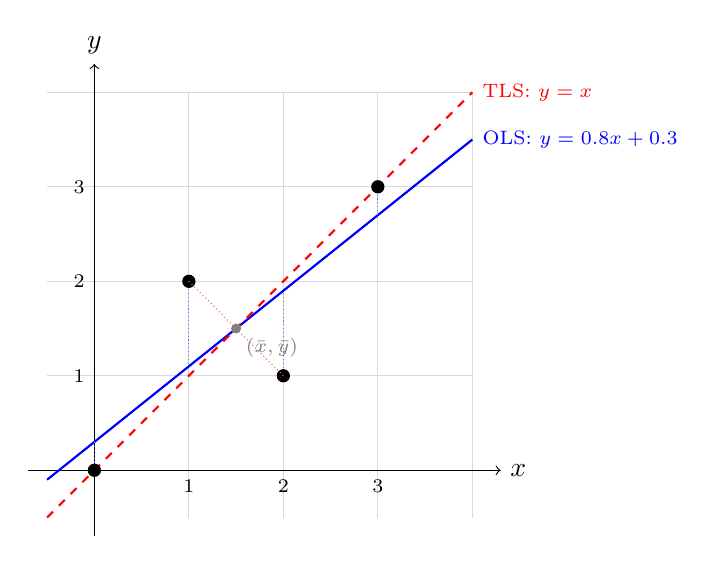
\begin{tikzpicture}[scale=1.2]
  \draw[gray!30] (-0.5,-0.5) grid (4,4);
  \draw[->] (-0.7,0) -- (4.3,0) node[right] {$x$};
  \draw[->] (0,-0.7) -- (0,4.3) node[above] {$y$};
  \foreach \t in {1,2,3} {\node[below,font=\scriptsize] at (\t,0) {$\t$}; \node[left,font=\scriptsize] at (0,\t) {$\t$};}
  \draw[blue,thick] (-0.5,-0.1) -- (4,3.5) node[right,font=\scriptsize] {OLS: $y=0.8x+0.3$};
  \draw[red,thick,dashed] (-0.5,-0.5) -- (4,4) node[right,font=\scriptsize] {TLS: $y=x$};
  \foreach \x/\y in {0/0,1/2,2/1,3/3} {
    \draw[blue!60,densely dotted] (\x,\y) -- (\x,0.8*\x+0.3);
    \fill (\x,\y) circle (2pt);
  }
  \draw[red!60,densely dotted] (1,2) -- (1.5,1.5);
  \draw[red!60,densely dotted] (2,1) -- (1.5,1.5);
  \fill[gray] (1.5,1.5) circle (1.5pt) node[below right,font=\scriptsize] {$(\bar x,\bar y)$};
\end{tikzpicture}
\caption{Data, OLS line (blue) with its vertical residuals, and TLS line (red) with its perpendicular residuals.}
\end{figure}
The two methods minimize different errors. OLS minimizes \emph{vertical} distances: it treats $x$ as exact and puts all the error in $y$. TLS minimizes \emph{perpendicular} distances, treating $x$ and $y$ the same way. The data are symmetric about $y=x$, so TLS returns exactly $y=x$. The OLS slope $m=S_{xy}/S_{xx}=4/5=0.8$ is pulled toward $0$ by the scatter in $y$. Both lines pass through the centroid $(1.5,1.5)$.

\subsection*{(d)}
\textbf{Total least squares.} When the noise in $x$ and $y$ is independent with equal variance, the error is isotropic. The best estimate (the maximum-likelihood fit) then minimizes perpendicular distance, which is what TLS does. TLS also does not depend on how the coordinate axes are oriented, and it handles vertical edges, where OLS fails because the slope is infinite.

%=====================================================================
\section*{Question 4}
%=====================================================================
Code: \texttt{hw3\_q4.py} (Appendix). TLS uses the smallest eigenvector of the covariance matrix, as in Question 3(b).

\subsection*{(a)}
For all 20 points: $(\bar x,\bar y)=(4.85,\,8.85)$, $\Sigma=\begin{bmatrix}43.43 & 3.88\\3.88 & 62.83\end{bmatrix}$, with eigenvalues $42.68$ and $63.57$.
\[
-0.9820\,x + 0.1890\,y + 3.0900 = 0 \quad(y = 5.196x - 16.349).
\]
\begin{figure}[H]\centering
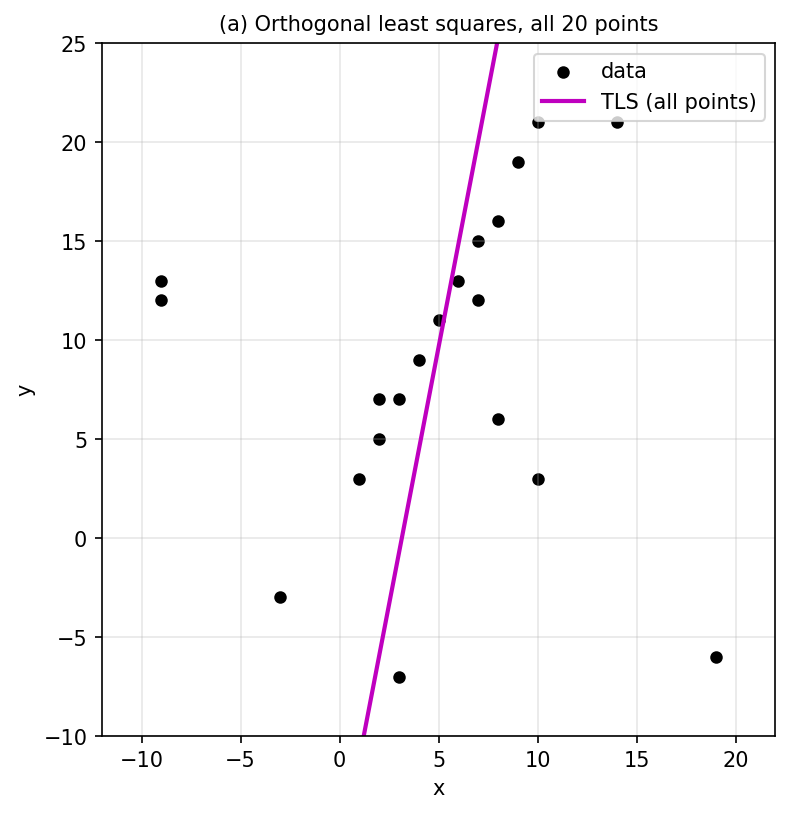
\includegraphics[width=0.5\linewidth]{figures/q4a_tls_all.png}
\end{figure}

\subsection*{(b)}
The random seed is $0$. The inlier threshold is $1.5$, with $p=0.99$, $s=2$ and $N_{\max}=100$. Whenever the best inlier count improves, the iteration limit becomes $\min\!\left(\lceil \ln(1-p)/\ln(1-w^2)\rceil,\,100\right)$:
\begin{center}
\begin{tabular}{cccc}\toprule
Iteration & Inliers (new best) & $w$ & New limit $N$\\\midrule
1 & 4 & 0.20 & $\min(113,100)=100$\\
2 & 6 & 0.30 & 49\\
4 & 13 & 0.65 & 9\\\bottomrule
\end{tabular}
\end{center}
Iterations 6 and 8 also found 13 inliers, but with a larger sum of squared distances (5.12 and 3.31 vs.\ 3.19), so iteration 4 is kept as the best.

\begin{figure}[H]\centering
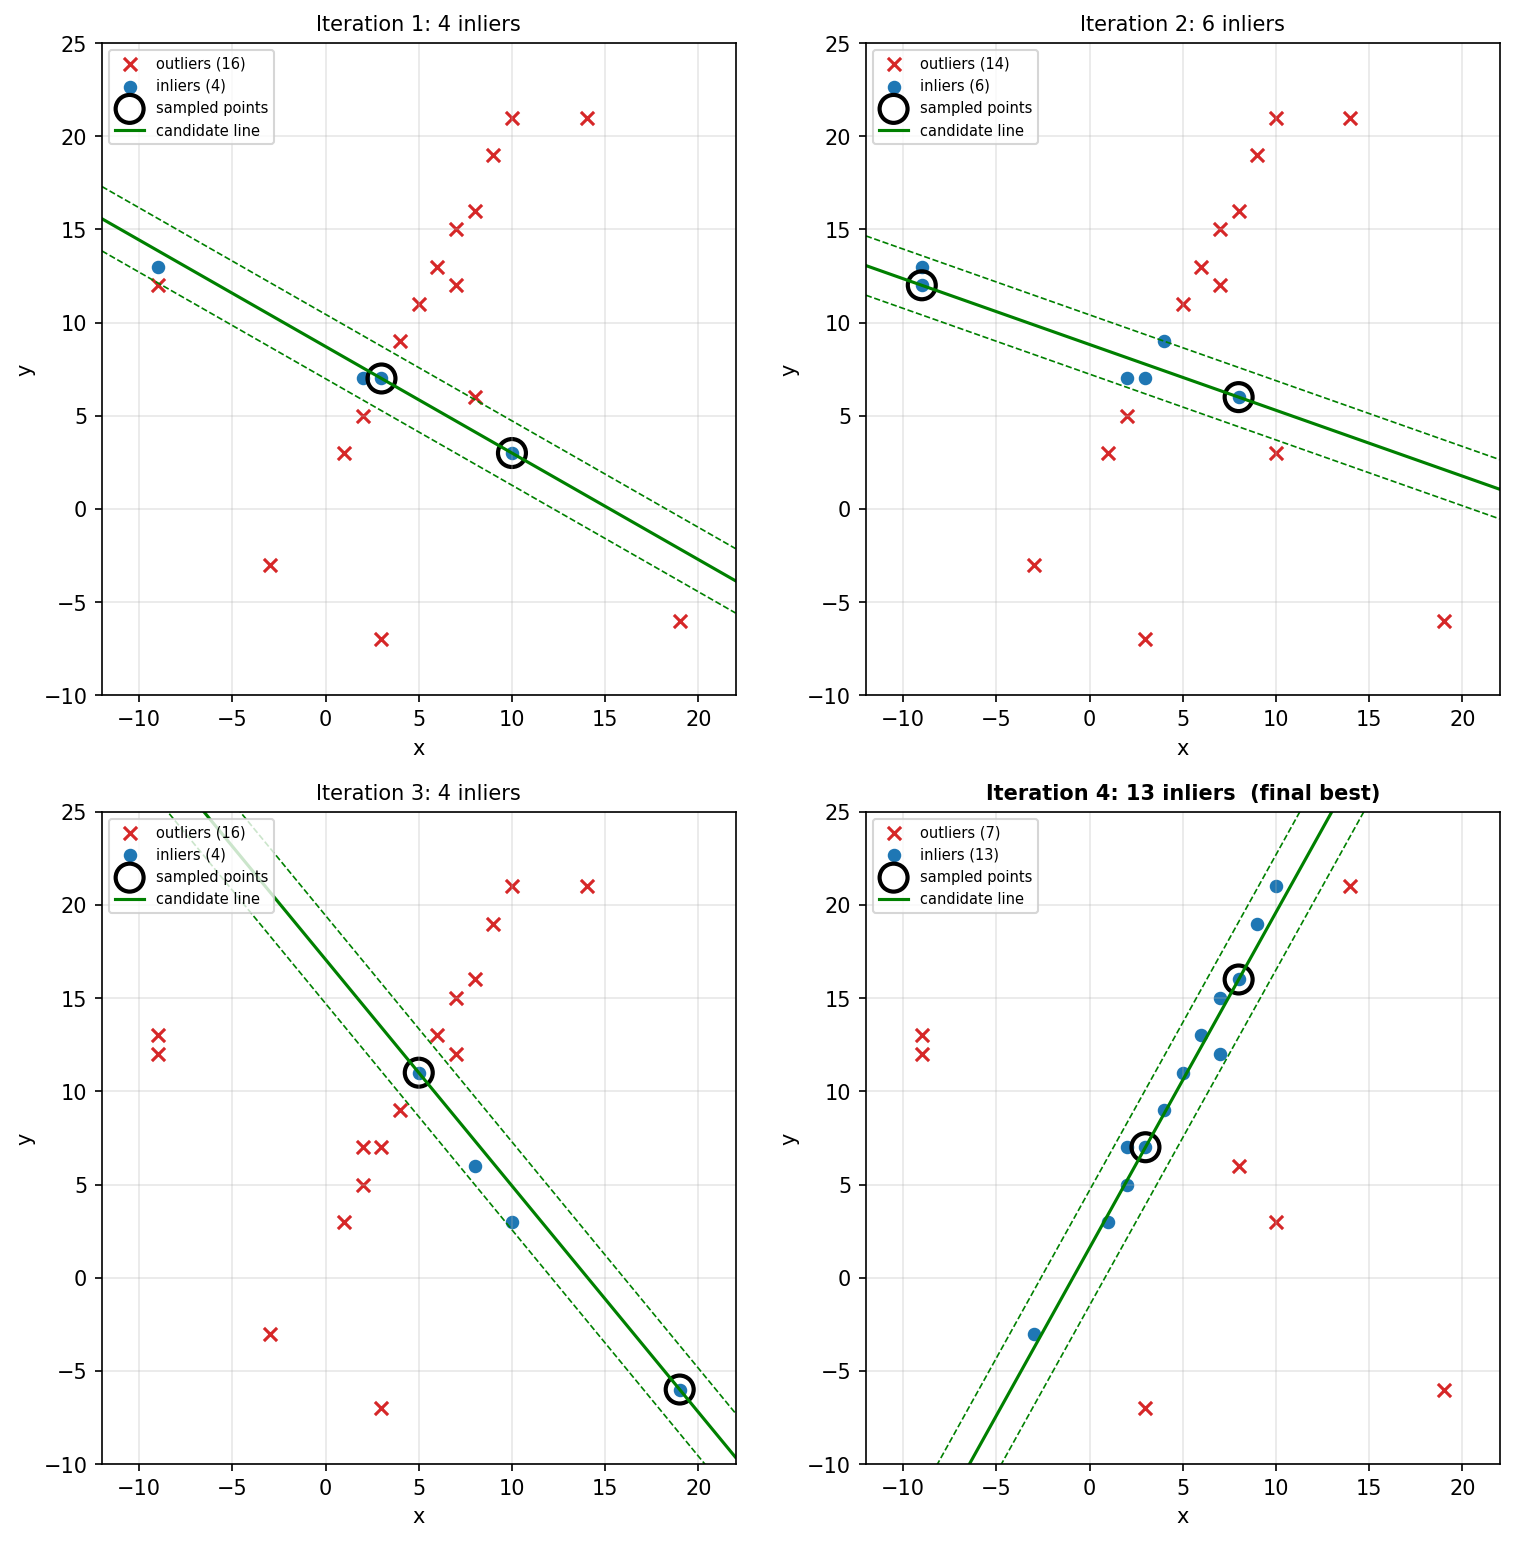
\includegraphics[width=0.85\linewidth]{figures/q4b_ransac_iterations.png}
\caption{RANSAC iterations 1--4. Black circles mark the two sampled points, the green line is the candidate, and the dashed lines show the $\pm1.5$ inlier band. Iteration 4 is the final best model.}
\end{figure}

\textbf{Final result:}
\begin{itemize}[leftmargin=*]
\item \textbf{13 inliers} and \textbf{7 outliers}. The outliers are $(19,-6)$, $(14,21)$, $(8,6)$, $(-9,12)$, $(3,-7)$, $(-9,13)$ and $(10,3)$.
\item Estimated inlier ratio: $w=0.65$.
\item \textbf{9 iterations} were performed in total.
\end{itemize}

\subsection*{(c)}
TLS on the 13 inliers gives eigenvalues $0.214$ and $53.47$, and the line
\[
-0.8785\,x + 0.4777\,y - 0.8386 = 0 \quad(y = 1.839x + 1.756).
\]
\begin{figure}[H]\centering
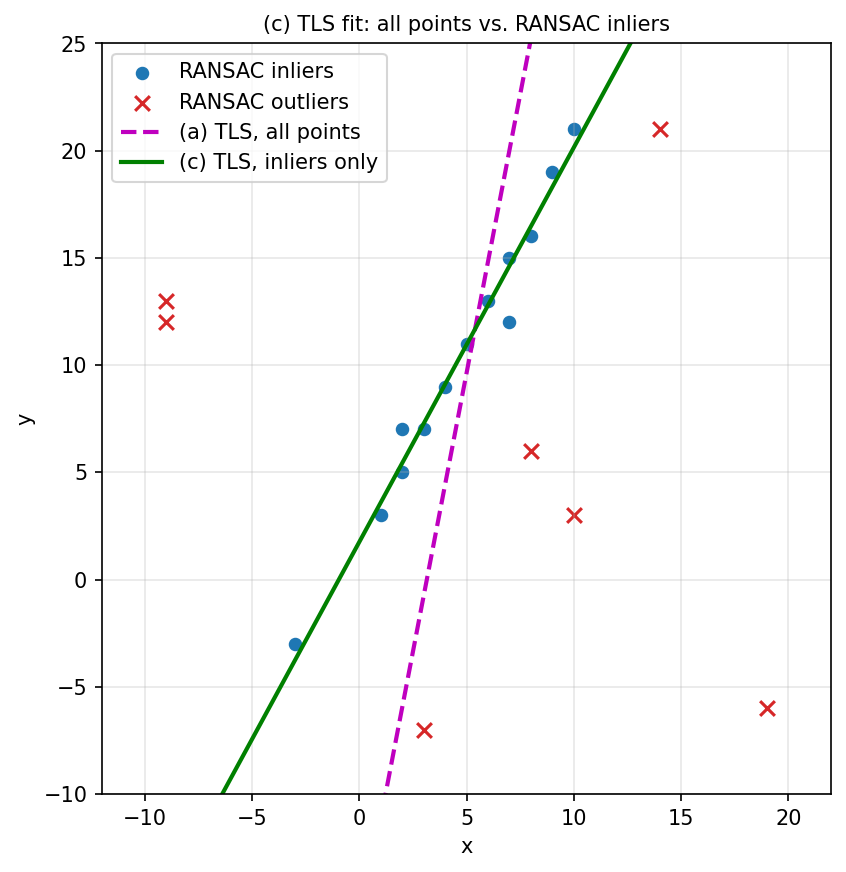
\includegraphics[width=0.55\linewidth]{figures/q4c_comparison.png}
\end{figure}
The inlier-only line follows the main group of points closely: the RMS distance of the inliers is $0.46$, compared with $2.30$ for the line from (a). The all-points line from (a) is much steeper (slope $5.2$ vs.\ $1.84$) and misses most of the data.

The problem is that least squares squares every residual, so points far from the line have a very large influence. The 7 outliers (35\% of the data) are spread far from the true line, for example $(19,-6)$, $(-9,12)$ and $(3,-7)$. They inflate the covariance in every direction, so its two eigenvalues ($42.7$ and $63.6$) are nearly equal, the "best" direction is poorly defined, and the fit is pulled away from the real structure. Once RANSAC removes the outliers, the smallest eigenvalue ($0.21$) is far below the largest ($53.5$), which shows a clear linear structure, and TLS recovers it accurately.

%=====================================================================
\appendix
\section*{Appendix: Code}
\subsection*{\texttt{hw3\_q4.py}}
\lstinputlisting{hw3_q4.py}

\end{document}
